\chapter{Anexos}

\section{Generación de proyecto Petalinux} \label{petalinux}

El paquete de software de PetaLinux proporciona al usuario las herramientas para configurar, construir y desplegar todos los componentes de software necesarios en las plataformas de Xilinx, que son:
\begin{itemize}
  \item \acrshort{FSBL}
  \item U-Boot
  \item ARM Trusted Firmware
  \item Linux
  \item Librerías y programas de usuario
  \item Hipervisor Xen
\end{itemize}


\subsection{Plataforma Hardware}
El primer paso para generar un proyecto de Petalinux es disponer de lo que en la nomenclatura Xilinx se denomina \textit{hardware platform specification}. Esta plataforma es el resultado de sintetizar el implementar el diseño definido en Vivado. Una vez que se ha generado el bitstream, se ha de exportar la plataforma, lo que genera un fichero \textit{.hdf} que contiene toda la información (configuración de \acrshort{PS} y bitstream para \acrshort{PL}) que nesecitan las herramientas de Xilinx para poder desarrollar software.

\subsection{Creación de proyecto}
Es necesario cargar las variables de entorno necesarias a fin de poder utilizar las herramientas del paquete de software PetaLinux en el host. Para ello es necesario introducir el siguiente comando (el texto entre signos < > debe ser sustituido por lo que corresponda según la instalción):\\

\begin{lstlisting}[style=CStyle]
alex@xubuntu16:~/workspace/ultrazed_hyp_1$ source <ruta_hasta_instalacion_petalinux>/settings.sh
\end{lstlisting}

Una vez hecho esto, el proyecto PetaLinux se crea con el siguiente comando en el que se le indica la plataforma (zynqMP para los MPSoC) y el nombre del proyecto, ultrazed\_hyp\_1.

\begin{lstlisting}[style=CStyle]
alex@xubuntu16:~/workspace/ultrazed_hyp_1$ petalinux-create --type project --template zynqMP --name ultrazed_hyp_1
\end{lstlisting}


\subsection{Importar plataforma hardware}

Una vez está creado el proyecto, a fin de importar la plataforma hardware previamente generada con Vivado, se ejecuta lo siguiente en la shell:

\begin{lstlisting}[style=CStyle]
alex@xubuntu16:~/workspace/ultrazed_hyp_1$ petalinux-config --get-hw-description=<ruta_hasta_fichero_hdf_generado_por_vivado>
\end{lstlisting}

Si en el directorio especificado existe un fichero \textit{.hdf}, entonces PetaLinux importa toda la configuración que contiene y muestra una ventana como la siguiente en la que perimite al usuario modificar los parámetros para la generación de los binarios:\\

\begin{figure*}[!h]
	\centering
	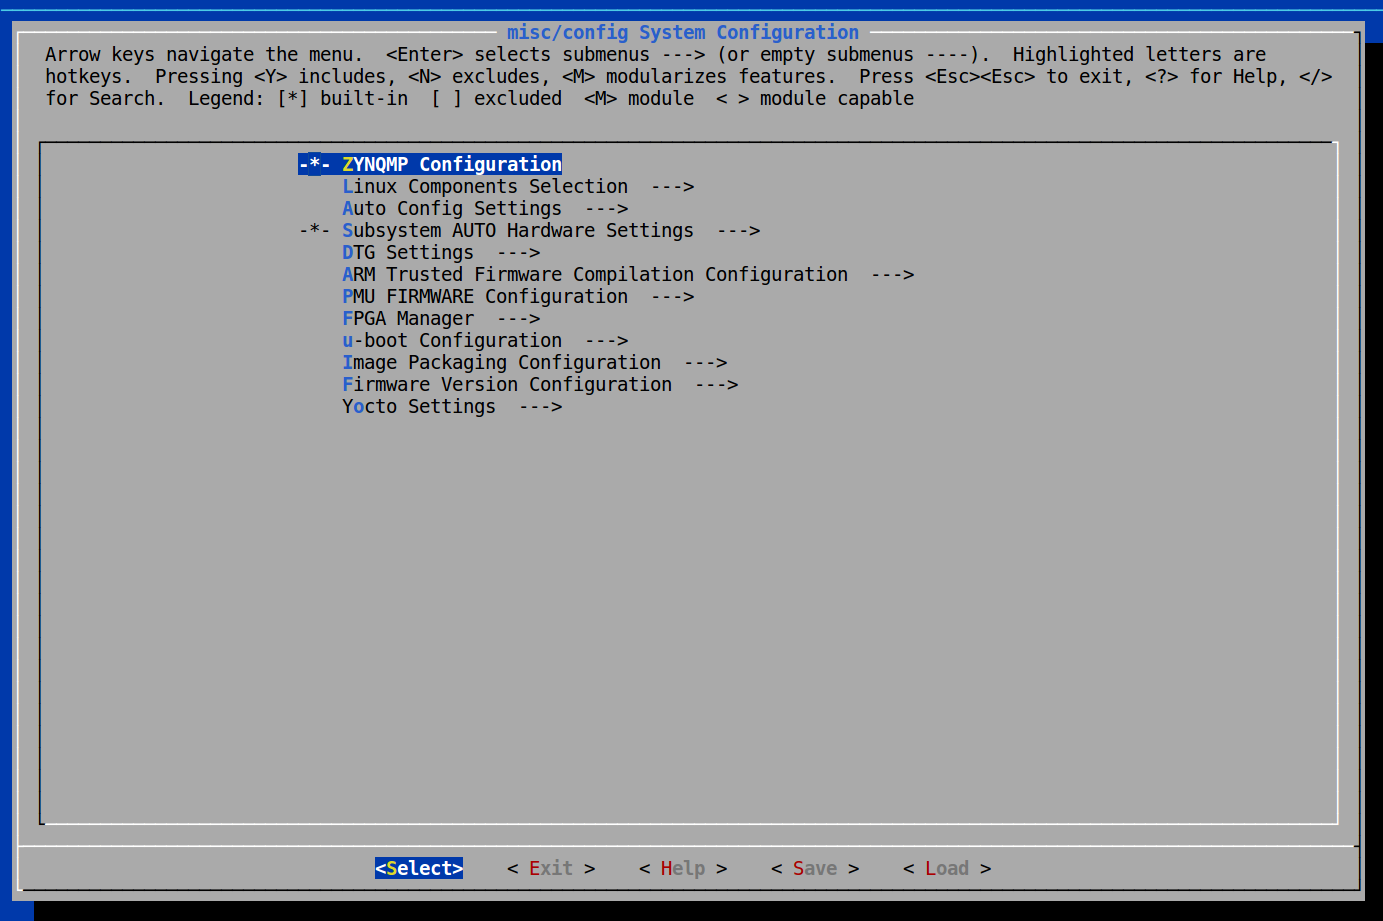
\includegraphics[width=0.70\textwidth]{recursos/petalinux_config_1.png}
	\caption{Configuración de proyecto PetaLinux}
	\label{fig:petalinux_config_1}
\end{figure*}



\subsection{Generar imagen de arranque}
